%\chapter{The Large Hadron Collider}
%%\section{Siliziumdetektoren}
%The LHC was build between 1998 and 2008 by the European Organization for Nuclear Research (CERN) in collaboration with 10000 scientist from over 100 countries
%and lies in a $\SI{27}{\kilo\meter}$ tunnel 175 metres underground in Switzerland near Geneva. It is a proton-proton synchrotron, which uses
%the systems to accelerate the protons before they are injected into the main accelerator. The linear particle accelerator LINAC 4 generates $\SI{160}{\mega\eV}$
%negative hydrogen ions and launches them into the Proton Synchrotron Booster (PSB). Here, the electrons are removed from the hydrogen ions, leaving only the nucleus
%consisting of one proton, which then enters the Super Proton Synchrotron (SPS). It increases the protons energy to $\SI{450}{\GeV}$ and feeds them to the
%LHC, where to opposing proton beams are accelerated. In the main ring,
%the protons are accumulated to bunches and accelerated to their maximum energy of $\SI{13}{\tera\eV}$ in 20 minutes.
%
%At four locations, the two proton beams
%are crossed, making it possible for them to collide. Around these interaction points, the four large experiments, ATLAS, CMS, LHCb and Alice are operated.
%Occasionaly lead nuclei are accelerated to study matter under extreme conditions at the ALICE experiment. The ATLAS and CMS experiment are general-purpose detectors for
%high energy physics. They differ on their technical design to achieve their goal and enable to corrobate each others results.
%LHCb is an asymmetric particle detector specialized in measuring the parameters of CP violation in B-meson decays.
%Further experiments at the LHC include TOTem, LHCf, MoEDAL and FASER, which focus on specialized research. Figure \ref{fig:lhc_aufbau} shows a schematic depiction
%of the LHC.
%
%\begin{figure}[H]
%  \centering
%  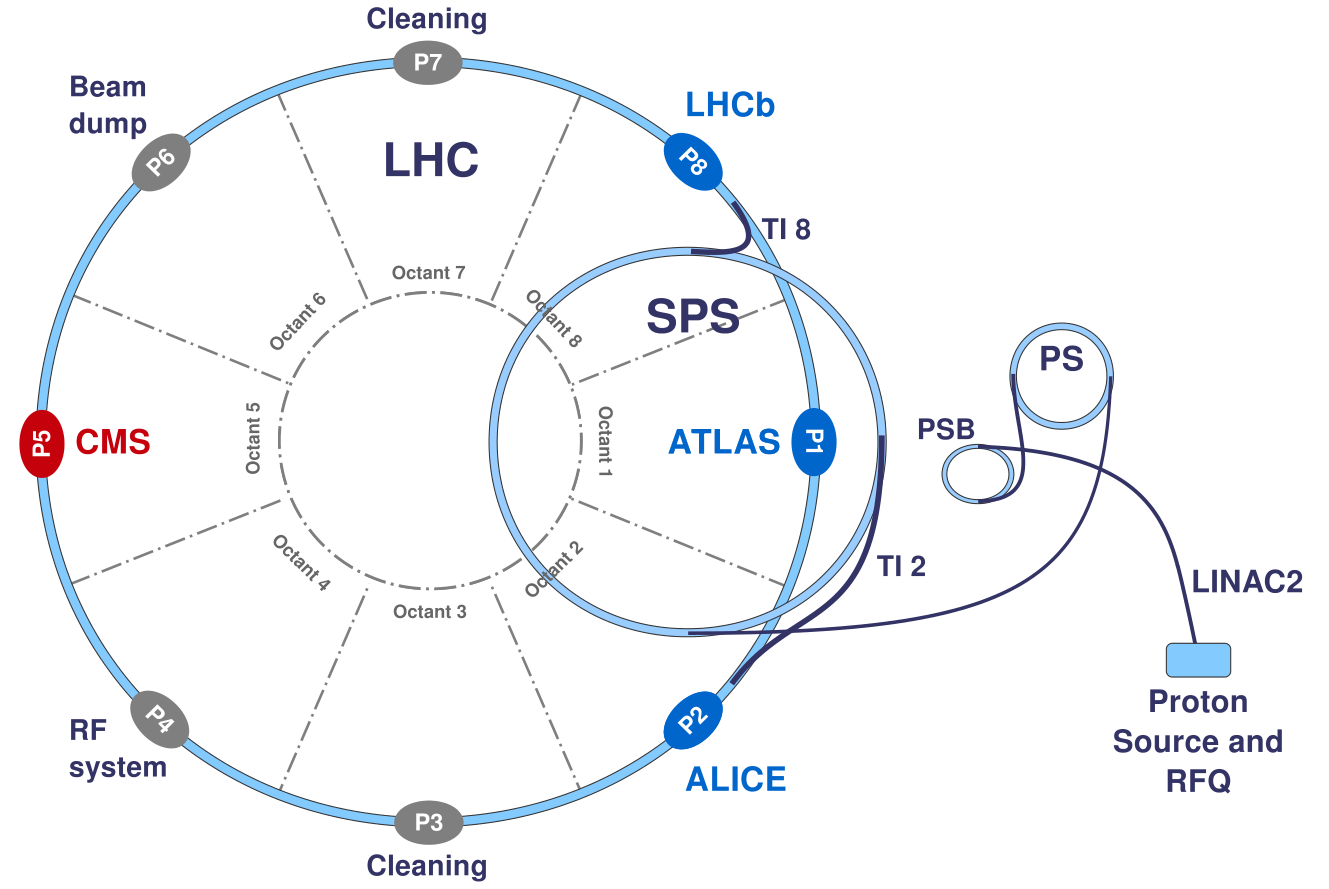
\includegraphics[height=0.4\textwidth]{images/lhc_aufbau.png}
%  \caption{Schematic representation of the CERN accelerator complex (not to scale)\cite{lhc_aufbau}.}
%  \label{fig:lhc_aufbau}
%\end{figure}
%
%After the second run from 2015 to 2018 followed the Long Shutdown 2 (LS2) until 2021 in order to upgrade the accelerator. The goal is to increase the luminosity by a factor of 10 by
%implementing High Luminosity Large Hadron Collider (HL-LHC) in the Long Shutdown 3 (LS3), which is planned to be operational in 2026. Figure \ref{fig:lhc_plan} shows the timeline
%of LHC programme.
%
%\begin{figure}
%  \centering
%  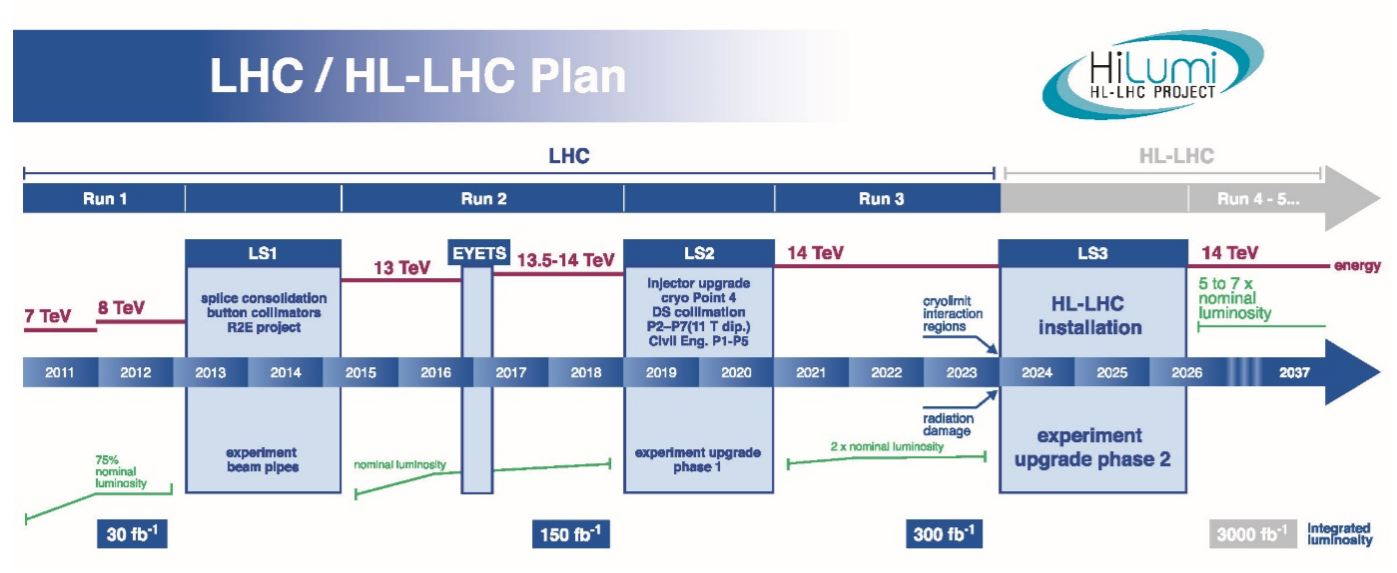
\includegraphics[height=0.4\textwidth]{images/lhc_plan.png}
%  \caption{Timeline of the operational phases and Shutdowns of the LHC. The energy of accelerated protons in each phase is shown in red and the luminosity in green \cite{lhc_plan}.}
%  \label{fig:lhc_plan}
%\end{figure}
%
%\section{The ATLAS detector}
%The ATLAS detector is the largest general-purpose detector with a length of $\SI{46}{\meter}$ and a diameter of $\SI{25}{\meter}$.
%It was designed to be a cylindric $4\pi$ detector, covering up most of the solid angle to detect particles flying in all directions.
%Both ATLAS and CMS detected the Higgs Boson in 2012 and thus prove the existence of the last missing particle of the standard model.
%Further goals of the detector is to search for beyond the standard model physics in the high energy domain, where current theories possibly break down.
%Top quarks, which were produced at the LHC in large amount of quantities for the first time, can be studied more precisely with the help of the ATLAS detector.
%
%The entire detector is made out of four different layers of detector systems, the Inner Detector, the electromagnetic and hadronic calorimeters
%and the muon spectrometer. Only a couple of centimeter away from the interaction point lies the Inner Detector with its purpose to track the produced charged particles.
%It is made of three subsequent components, with the innermost layer called the Pixel Detector and consists of three layers of silicon pixel detectors. The middle constituent
%is the Semiconductor Tracker (SRT) with a similar purpose. Here, four layers of silicon stripe detectors are used for detection, while they have a lower spatial resolution, a larger
%area can be covered with them more efficiently. The Transition Radiation Tracker (TRT) is the outermost component and uses straw detectors for tracking as well as materials with
%different refractive index inbetween the straws. Relativistic particles will produce transition radiation by traversing these materials, which enables particle
%identification, especially for light charged particles.
%A magnetic solenoid surrounding the Inner Detector produces a $\SI{2}{\tesla}$ magnetic field to curve the trajectories of charged particles in order to determine their
%momentum. \\
%The electromagnetic calorimeter is positioned outside the magnetic field and aims at absorbing electrons, positrons and photon induced
%electromagnetic showers in order to measure the energy of the initial particle. Lead and stainless steel serve as the energy absorbing material and liquid argon as the
%sampling material. Hadrons tend to traverse the electromagnetic calorimeter without losing all their energy, which is the reason the hadronic calorimeter comes after.
%It uses steel as sampling material and scintillating tiles to measure the energy. \\
%Because muons easily pass both calorimeters, the outermost detector system is the muon spectrometer consisting of silicon detectors to track the muons and three toroidal magnets
%building up a magnetic field for momentum measurement. Figure \ref{fig:atlas} ilustrates the ATLAS detector with its components.
%
%\begin{figure}
%  \centering
%  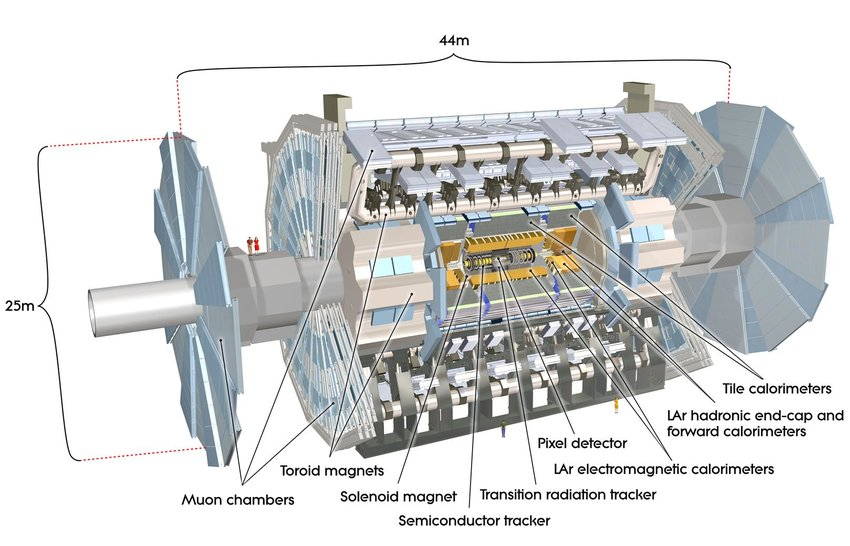
\includegraphics[height=0.5\textwidth]{images/atlas.png}
%  \caption{Illustration of the ATLAS detector and its subsequent components. Two Humans are depicted at the bottom for a size comparison \cite{atlas}.}
%  \label{fig:atlas}
%\end{figure}
%
%During the Long Shutdown 3 of the LHC, the ATLAS Inner Tracker (ITk) upgrade is planned to be installed. Its goal is to perform as good or better as the current detector, while
%withstanding the harsher environment of the HL-LHC.

\chapter{Radiation therapy}
Radiation therapies \cite{med} are medical treatments using ionising radiation mainly to kill cancer cells in patients. The ionising particles interact with the
cancer cells to damage their DNA causing cellular death. These treatments focus on cancer that is localised to one area inside the body. \\
The type of particle used in radiation therapy is crucial to the overall treatment due to their different interactions with the human body.
Photons are the most common particles being used for radiation therapy \cite{pbt}.
A newer alternative is proton therapy, having several advantages over conventional x-ray therapy, due to its different properties, which are explained in the following section.


\section{Proton therapy}
Proton therapy is external beam radiotherapy using a proton beam for irradiation.
While proton therapy centres have only been used since 1954 \cite{pct_history}, the technological
advance ensures the continual rise of hospitals offering proton therapy. \\
The proton therapy centres either use cyclotrons or synchrotrons to accelerate the protons.
For cyclotrons, protons are extracted from hydrogen atoms and accelerated with
a constant magnetic field outwards from the centre of the cyclotron until they reach a velocity of approximately 2/3 of the speed of light. Afterwards, the protons
are focused into the beamline by a magnet system. Synchrotrons use a variable,
high-frequency magnetic fields to focus protons on a circular path on which they are accelerated. While they
are not as compact as cyclotrons, they are able to produce protons of varying energies from $\SI{50}{\MeV}$ to $\SI{250}{\MeV}$ \cite{cyclo}. \\
Unlike protons, photons deposit most of their energy near the surface due to Compton scattering and pair production for energies
in the $\mathrm{MeV}$ regime \cite{compton}.
%Unlike photons, which tend to deposit most of their energy near the surface due to Compton scattering,
%protons undergo multiple Coulomb scattering inside matter without a significant energy deposition near the surface.
The energy loss $-\text{d}E$ of protons per distance $\text{d}x$ in this energy region can be described by the Bethe \mbox{formula \cite{bethe}}:
\begin{align}
  - \frac{dE}{dx} = \frac{4\pi}{m_e c^2}\left(\frac{e^2}{4\pi\epsilon_0}\right)^2\frac{nz^2}{\beta^2} \left[ \frac{1}{2} \ln{\left(\frac{2 m_e c^2 \beta^2}{I(1-\beta^2)}\right)} - \beta^2 \right]
\end{align}
Here, c is the speed of light,  $I$ is the mean excitation potential, $n$ is the electron density, $\epsilon_0$ is the vacuum permittivity, $e$ the electron charge,
$m_e$ the electron mass, and $\beta = v/c$.
This means that the energy loss is inversely proportional to the square of their velocity, which causes them to deposit most of their energy on the last millimeters of their path.
This behaviour is called the Bragg peak and is shown in Figure \ref{fig:bragg}.
Regulating the energy of the protons allows for precise control of the Bragg peak depth inside
the human body. Thus, having multiple proton energies in the proton beam by using absorbers between
the accelerator and the patient enables a uniform energy deposition inside the target volume, causing a spread-out Bragg peak (SOBP) \cite{sobp}.

\begin{figure}
  \centering
  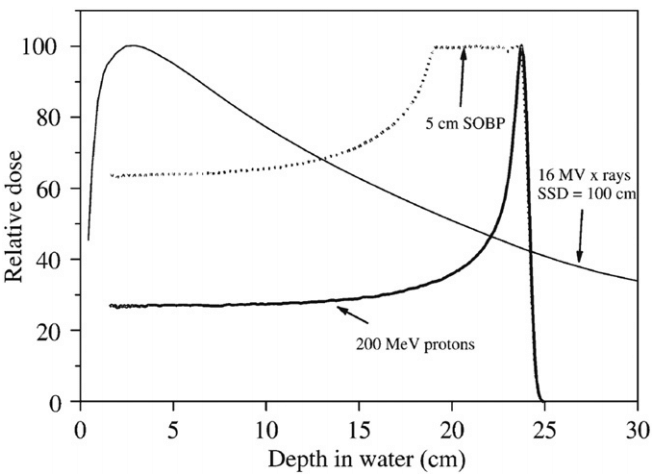
\includegraphics[height=0.6\textwidth]{images/tiefendosis.png}
  \caption{A Radiation dose of unmodulated $\SI{200}{\mega\eV}$ protons and with a $\SI{5}{\centi\meter}$ spread-out Bragg peak
  as a function of the penetration depth in water. In comparison, the energy deposition of a $\SI{16}{\mega\eV}$ x-ray beam \cite{bragg}.}
  \label{fig:bragg}
\end{figure}
Due to this property, protons enable the irradiation of tumors with greater precision than with
x-rays, as surrounding healthy tissue is less damaged, especially behind the tumor. Figure \ref{fig:risk} shows the irradiated areas during treatment of brain cancer
for conventional radiation and
proton therapy to emphasise their differences.

\begin{figure}
  \centering
  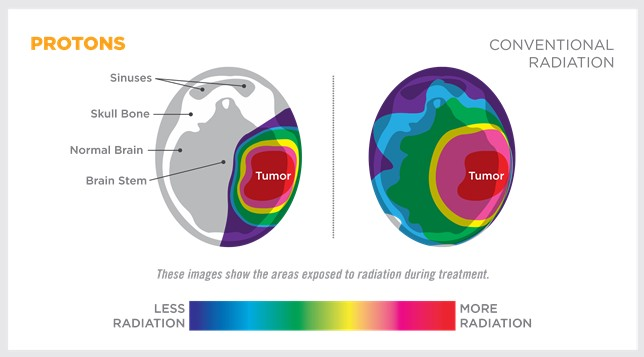
\includegraphics[height=0.5\textwidth]{images/risk.png}
  \caption{Irradiated region for protons and x-rays to treat a brain tumor. The irradiation for proton therapy is far more precise and damages less healthy tissue than
  x-ray therapy \cite{brain}.}
  \label{fig:risk}
\end{figure}


\section{Computed tomography} \label{sec:ct}
To irradiate a patient safely and efficiently it is necessary to create an irradiation plan by localising the tumor and the surrounding healthy tissue. In order to do so, a computed
tomography (CT) scan is performed using a particle beam to create an image of the region encompassing the tumor. For x-ray therapy as well as proton therapy x-ray CT scans
are used primarily. \\
To create an image, the patient lies within a gantry, which generates x-ray beams to irradiate the specific volume. The gantry also
includes a row of detectors measuring the photons after traversing the human body. Due to the fact that each tissue absorbs
x-rays differently, a projection of the irradiated volume can be created. By rotating the x-ray tube and the detectors, projections are created from many different angles around the patient.
Unlike in radiography, where two-dimensional projections are produced, CT scan measurements are one-dimensional absorption profiles. The sum of the profiles contains
the entire information of the inside structure, but cannot be interpreted directly. Projections and the original three-dimensional structure are connected through
the inverse radon transformation. \\
An implementation of that algorithm is the filtered back \mbox{projection \cite{back_projection}:}
\begin{align}
  f(x,y) = \int_0^{\pi} \left(\int_{-\infty}^{\infty} p_{\phi}(z') \cdot g(z - z') \mathrm{d}z'\right) \mathrm{d}\phi
\end{align}
where $f(x,y)$ is the original image, $p_{\phi}(z)$ the projection in the direction of the angle $\phi$ and $g(z)$ a high-pass filter. However, the inverse
radon transformation is an ill-posed problem, which demands an irregular filter kernel $g(z)$. To solve this problem in praxis, a fast convolution algorithm is used for the
filtered back projection. This means that the projection is multiplied with the high-pass filter in Fourier space, where each frequency component is weighted proportional to its
absolute value. In the end, each one-dimensional projection is stretched into two dimensions and rotated around the angle $-\phi$. The sum over all projections will yield the
final image.


\section{Proton computed tomography}
Creating irradiation plans for proton therapy with x-ray computed tomography images causes large uncertainties due to the different stopping powers of the particles.
To compensate for the differences, a range uncertainty margin is applied to the prescribed range, which increases with greater travel distance through the body. This
method is shown in Figure \ref{fig:paganetti}. These uncertainty margins caused by the conversion of x-rays to protons for the radiation plan can be prevented by creating a proton computed tomography (pCT) image.
Since the position of the protons energy deposition has to be determined as precisely as possible to minimise the damage inflicted to healthy tissue, a computed tomography scan using protons
is a promising alternative to \mbox{conventional CT}.

\begin{figure}
  \centering
  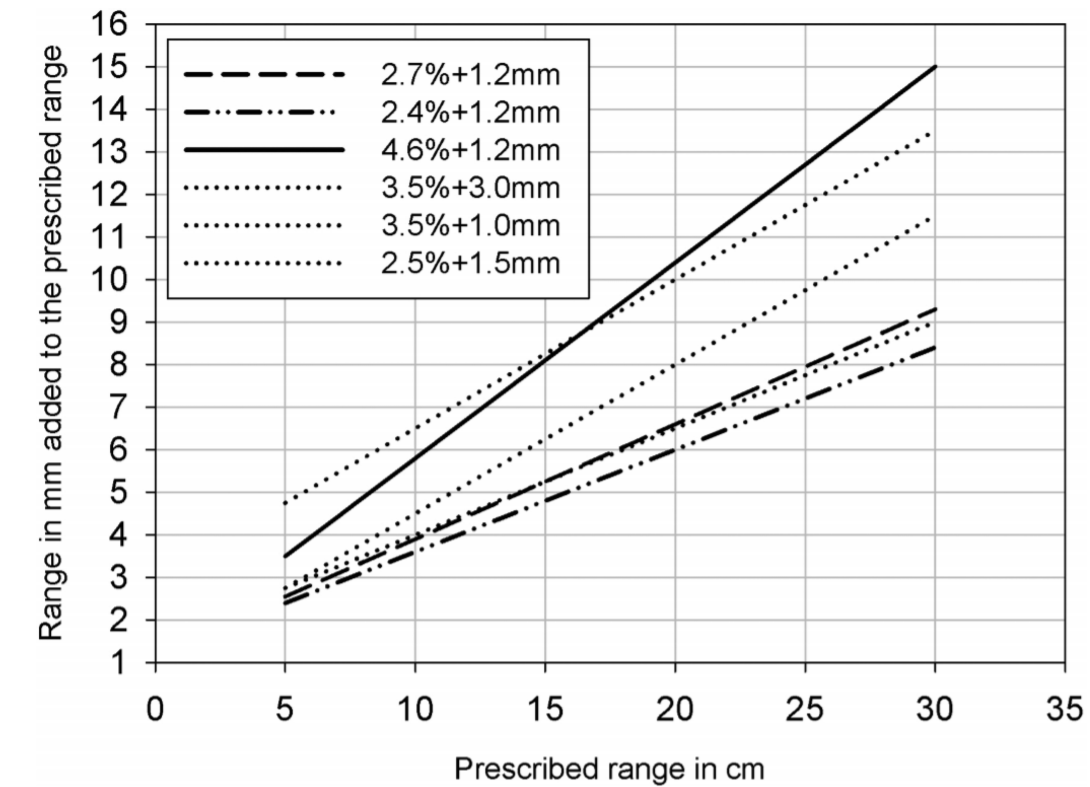
\includegraphics[height=0.5\textwidth]{images/prescription.png}
  \caption{Applied uncertainty margins at the Massachusetts General Hospital (3.5\,\% +
1mm), the MD Anderson Proton Therapy Centre in Houston (3.5\,\% + 3mm), the Loma Linda
University Medical Centre (3.5\,\% + 3mm), the Roberts Proton Therapy Centre at the
University of Pennsylvania (3.5\,\% + 3mm), and the University of Florida Proton Therapy
Institute (2.5\,\% + 1.5mm), shown as dotted lines. Dashed-dotted and dashed line: Uncertainty margin with and without the use of Monte Carlo dose calculation.
The solid-line describes the safety margin for complex geometries without Monte Carlo dose calculation \cite{paganetti}.}
  \label{fig:paganetti}
\end{figure}

Creating an image with proton CT is similar to conventional CTs. A proton beam deposits energy in the patient and the
protons remaining energy is then measured with a calorimeter system behind the patient to gain information about the composition of the tissue. A projection can be created,
if the tracks of the protons are reconstructed. However, due to multiple Coulomb scatterings of the protons inside the patient, the spatial resolution will decrease in comparison
to conventional ct. In order to take the multiple Coulomb scattering into account, a most likely path formalism is necessary to model the path of the proton inside the patient \cite{mlp}.
Numerous projections are created by varying the angle of the proton beam with respect to the target. The entire setup is schematically shown in Figure \ref{fig:proton_ct}.

\begin{figure}
  \centering
  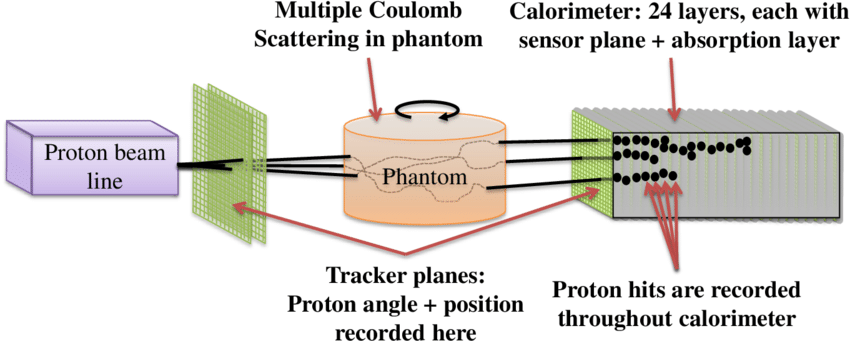
\includegraphics[height=0.35\textwidth]{images/proton_ct.png}
  \caption{Procedure of the proton computed tomography. The tracker planes are used to reconstruct the proton tracks and the calorimeter to measure their remaining energy.
  The phantom is the placeholder of a patient \cite{proton_ct}.}
  \label{fig:proton_ct}
\end{figure}

The different projections can then be reconstructed to a complete image of the irradiated volume as explained in section \ref{sec:ct}.
This thesis focuses on the track reconstruction of the low energy protons used in proton computed tomography and whether they can be reconstructed accurately.
In the following chapter, the track reconstruction of particles is addressed in more detail.
